%%%%%%%%%%%%%%%%%%%%%%%%%%%%%%%%%%%%%%%%%
% Tufte-Style Book (Documentation Template)
% LaTeX Template
% Version 1.0 (5/1/13)
%
% This template has been downloaded from:
% http://www.LaTeXTemplates.com
%
% Original author:
% The Tufte-LaTeX Developers (tufte-latex.googlecode.com)
%
% License:
% Apache License (Version 2.0)
%
% IMPORTANT NOTE:
% In addition to running BibTeX to compile the reference list from the .bib
% file, you will need to run MakeIndex to compile the index at the end of the
% document.
%
%%%%%%%%%%%%%%%%%%%%%%%%%%%%%%%%%%%%%%%%%

%----------------------------------------------------------------------------------------
%	PACKAGES AND OTHER DOCUMENT CONFIGURATIONS
%----------------------------------------------------------------------------------------

\documentclass{tufte-book} % Use the tufte-book class which in turn uses the tufte-common class

\hypersetup{colorlinks} % Comment this line if you don't wish to have colored links
\usepackage{hyperref}
\usepackage{microtype} % Improves character and word spacing
\usepackage[utf8]{inputenc}
\usepackage{listings}
\usepackage{lipsum} % Inserts dummy text

\usepackage{booktabs} % Better horizontal rules in tables

\usepackage{graphicx} % Needed to insert images into the document
\graphicspath{{graphics/}} % Sets the default location of pictures
\setkeys{Gin}{width=\linewidth,totalheight=\textheight,keepaspectratio} % Improves figure scaling

%\usepackage{tikz-cd}
\usepackage{tikz}
\usetikzlibrary{patterns}

\usepackage{fancyvrb} % Allows customization of verbatim environments
\fvset{fontsize=\normalsize} % The font size of all verbatim text can be changed here

\newcommand{\hangp}[1]{\makebox[0pt][r]{(}#1\makebox[0pt][l]{)}} % New command to create parentheses around text in tables which take up no horizontal space - this improves column spacing
\newcommand{\hangstar}{\makebox[0pt][l]{*}} % New command to create asterisks in tables which take up no horizontal space - this improves column spacing

\usepackage{xspace} % Used for printing a trailing space better than using a tilde (~) using the \xspace command

\newcommand{\monthyear}{\ifcase\month\or January\or February\or March\or April\or May\or June\or July\or August\or September\or October\or November\or December\fi\space\number\year} % A command to print the current month and year

\newcommand{\openepigraph}[2]{ % This block sets up a command for printing an epigraph with 2 arguments - the quote and the author
\begin{fullwidth}
\sffamily\large
\begin{doublespace}
\noindent\allcaps{#1}\\ % The quote
\noindent\allcaps{#2} % The author
\end{doublespace}
\end{fullwidth}
}

\newcommand{\blankpage}{\newpage\hbox{}\thispagestyle{empty}\newpage} % Command to insert a blank page

\usepackage{units} % Used for printing standard units

\newcommand{\hlred}[1]{\textcolor{Maroon}{#1}} % Print text in maroon
\newcommand{\hangleft}[1]{\makebox[0pt][r]{#1}} % Used for printing commands in the index, moves the slash left so the command name aligns with the rest of the text in the index 
\newcommand{\hairsp}{\hspace{1pt}} % Command to print a very short space
\newcommand{\ie}{\textit{i.\hairsp{}e.}\xspace} % Command to print i.e.
\newcommand{\eg}{\textit{e.\hairsp{}g.}\xspace} % Command to print e.g.
\newcommand{\na}{\quad--} % Used in tables for N/A cells
\newcommand{\measure}[3]{#1/#2$\times$\unit[#3]{pc}} % Typesets the font size, leading, and measure in the form of: 10/12x26 pc.
\newcommand{\tuftebs}{\symbol{'134}} % Command to print a backslash in tt type in OT1/T1

\providecommand{\XeLaTeX}{X\lower.5ex\hbox{\kern-0.15em\reflectbox{E}}\kern-0.1em\LaTeX}
\newcommand{\tXeLaTeX}{\XeLaTeX\index{XeLaTeX@\protect\XeLaTeX}} % Command to print the XeLaTeX logo while simultaneously adding the position to the index

\newcommand{\doccmdnoindex}[2][]{\texttt{\tuftebs#2}} % Command to print a command in texttt with a backslash of tt type without inserting the command into the index

\newcommand{\doccmddef}[2][]{\hlred{\texttt{\tuftebs#2}}\label{cmd:#2}\ifthenelse{\isempty{#1}} % Command to define a command in red and add it to the index
{ % If no package is specified, add the command to the index
\index{#2 command@\protect\hangleft{\texttt{\tuftebs}}\texttt{#2}}% Command name
}
{ % If a package is also specified as a second argument, add the command and package to the index
\index{#2 command@\protect\hangleft{\texttt{\tuftebs}}\texttt{#2} (\texttt{#1} package)}% Command name
\index{#1 package@\texttt{#1} package}\index{packages!#1@\texttt{#1}}% Package name
}}

\newcommand{\doccmd}[2][]{% Command to define a command and add it to the index
\texttt{\tuftebs#2}%
\ifthenelse{\isempty{#1}}% If no package is specified, add the command to the index
{%
\index{#2 command@\protect\hangleft{\texttt{\tuftebs}}\texttt{#2}}% Command name
}
{%
\index{#2 command@\protect\hangleft{\texttt{\tuftebs}}\texttt{#2} (\texttt{#1} package)}% Command name
\index{#1 package@\texttt{#1} package}\index{packages!#1@\texttt{#1}}% Package name
}}

% A bunch of new commands to print commands, arguments, environments, classes, etc within the text using the correct formatting
\newcommand{\docopt}[1]{\ensuremath{\langle}\textrm{\textit{#1}}\ensuremath{\rangle}}
\newcommand{\docarg}[1]{\textrm{\textit{#1}}}
\newenvironment{docspec}{\begin{quotation}\ttfamily\parskip0pt\parindent0pt\ignorespaces}{\end{quotation}}
\newcommand{\docenv}[1]{\texttt{#1}\index{#1 environment@\texttt{#1} environment}\index{environments!#1@\texttt{#1}}}
\newcommand{\docenvdef}[1]{\hlred{\texttt{#1}}\label{env:#1}\index{#1 environment@\texttt{#1} environment}\index{environments!#1@\texttt{#1}}}
\newcommand{\docpkg}[1]{\texttt{#1}\index{#1 package@\texttt{#1} package}\index{packages!#1@\texttt{#1}}}
\newcommand{\doccls}[1]{\texttt{#1}}
\newcommand{\docclsopt}[1]{\texttt{#1}\index{#1 class option@\texttt{#1} class option}\index{class options!#1@\texttt{#1}}}
\newcommand{\docclsoptdef}[1]{\hlred{\texttt{#1}}\label{clsopt:#1}\index{#1 class option@\texttt{#1} class option}\index{class options!#1@\texttt{#1}}}
\newcommand{\docmsg}[2]{\bigskip\begin{fullwidth}\noindent\ttfamily#1\end{fullwidth}\medskip\par\noindent#2}
\newcommand{\docfilehook}[2]{\texttt{#1}\index{file hooks!#2}\index{#1@\texttt{#1}}}
\newcommand{\doccounter}[1]{\texttt{#1}\index{#1 counter@\texttt{#1} counter}}
\usepackage{pst-node}
\usepackage{makeidx} % Used to generate the index
\makeindex % Generate the index which is printed at the end of the document

% This block contains a number of shortcuts used throughout the book
\newcommand{\vdqi}{\textit{VDQI}\xspace}
\newcommand{\pfds}{\textbf{\textit{PFDS}}\xspace}
\newcommand{\fp}{\textbf{\textit{FP}}\xspace}
\newcommand{\ei}{\textit{EI}\xspace}
\newcommand{\ve}{\textit{VE}\xspace}
\newcommand{\be}{\textit{BE}\xspace}
\newcommand{\VDQI}{\textit{The Visual Display of Quantitative Information}\xspace}
\newcommand{\EI}{\textit{Envisioning Information}\xspace}
\newcommand{\VE}{\textit{Visual Explanations}\xspace}
\newcommand{\BE}{\textit{Beautiful Evidence}\xspace}
\newcommand{\TL}{Tufte-\LaTeX\xspace}

\definecolor{punct}{rgb}{0.0,0.24313725490196078,1.0}
\definecolor{numb}{rgb}{0.0,0.24313725490196078,1.0}
\usepackage[svgnames]{xcolor} % Enabling colors by their 'svgnames'
%----------------------------------------------------------------------------------------
%	BOOK META-INFORMATION
%----------------------------------------------------------------------------------------

\title{Characterization of topological models for distributed computing with logical systems.} % Title of the book

\author{Fabián Romero} % Author

\publisher{Posgrado en Ciencia e Ingeniería de la Computación} % Publisher

%----------------------------------------------------------------------------------------

\begin{document}
\lstdefinelanguage{json}{
    basicstyle=\normalfont\ttfamily,
    numbers=left,
    framexleftmargin=0pt,
    xleftmargin=2em,
    numberstyle=\scriptsize,
    stepnumber=1,
    numbersep=8pt,
    showstringspaces=false,
    breaklines=true,
    morecomment=[s]{/*}{*/},
    morecomment=[l]--,
    frame=lines,
%    backgroundcolor=\color{background},
    literate=
     *{0}{{{\color{numb}0}}}{1}
      {1}{{{\color{numb}1}}}{1}
      {2}{{{\color{numb}2}}}{1}
      {3}{{{\color{numb}3}}}{1}
      {4}{{{\color{numb}4}}}{1}
      {5}{{{\color{numb}5}}}{1}
      {6}{{{\color{numb}6}}}{1}
      {7}{{{\color{numb}7}}}{1}
      {8}{{{\color{numb}8}}}{1}
      {9}{{{\color{numb}9}}}{1}
      {:}{{{\color{punct}{:}}}}{1}
      {,}{{{\color{punct}{,}}}}{1}
      {\{}{{{\color{delim}{\{}}}}{1}
      {\}}{{{\color{delim}{\}}}}}{1}
      {[}{{{\color{delim}{[}}}}{1}
      {]}{{{\color{delim}{]}}}}{1},
}
\maketitle % Print the title page

%----------------------------------------------------------------------------------------
%	COPYRIGHT PAGE
%----------------------------------------------------------------------------------------
\newpage
\begin{fullwidth}
~\vfill
\thispagestyle{empty}
\setlength{\parindent}{0pt}
\setlength{\parskip}{\baselineskip}
Copyright \copyright\ \the\year\ \thanklessauthor

\par\smallcaps{Published by \thanklesspublisher}

\par\smallcaps{tufte-latex.googlecode.com}

\par Licensed under the Apache License, Version 2.0 (the ``License''); you may not use this file except in compliance with the License. You may obtain a copy of the License at \url{http://www.apache.org/licenses/LICENSE-2.0}. Unless required by applicable law or agreed to in writing, software distributed under the License is distributed on an \smallcaps{``AS IS'' BASIS, WITHOUT WARRANTIES OR CONDITIONS OF ANY KIND}, either express or implied. See the License for the specific language governing permissions and limitations under the License.\index{license}

\end{fullwidth}

%----------------------------------------------------------------------------------------
\tableofcontents % Print the table of contents

%----------------------------------------------------------------------------------------
%	INTRODUCTION
%----------------------------------------------------------------------------------------
\chapter{Summary} 

A distributed system (DS) can be defined as a collection of processes executing 
a protocol (algorithm) within a communicating environment. 
Studying such operational description to find properties on DS has shown to be 
a complex task, even when the number of processes and connections is limited 
and/or following simple patterns. It's complexity comes for the number of possible 
interactions of their elements  and the dynamics of such interactions.

On it's seminal paper \cite{Herlihy1999} Herlihy  introduced a characterization of DS, 
mapping the specifics of such protocols and environments to a topological structure.
In this combinatorial description all possible events on the dynamic of the interactions 
are represented simultaneously on a single topological structure.
Such approach it is a deliberated trade off. Interchanging one model with complex 
dynamics and relatively simple elements for other with complex elements but static.

This technique for the analysis of distributed systems has gained significant traction 
and has become widely used.
Gaining from a large set of topology results that can be immediately applied, and, as 
he argues. Our minds are much better equipped for analyzing static entities even when they are very complex than for dynamic ones even if they are sparse.

(DS) have been studied from many areas and multiple angles, in particular, it has been 
covered on many diferent logic aproaches, epistemic logic \cite{Meyer:1995} is a natural formulation for 
them, there's a great tradition on the field of artificial inteligence associating several logics to the study of (DS) \cite{HandbookAI1}, and many other logics as multi modal logic \cite{Hintikka1962}, dynamic epistemic logic \cite{Ditmarsch:2007}, among many others.
\newpage

Those works are intended to comprehend communications, epistemic development and 
behavior of such systems from an operational point of view.

In this work, we intend to mimic the aproach taken by Herlihy, and to map their topological models to kripke structures, the computational power of those processes to axioms, semantics and inference  rules of a formal logic system. And to transform some of the results to logical equivalents, in order to develop techniques, methods and insight that can help to solve other problems or to be able to find other characteristics on the resulting models, such as completion, consistency, decidability, etc.

%
%Ever since Herlihy  introduced it. The topological characterization for distributed computing has gained significant traction. And has become a widely used technique for the analysis of distributed systems. In which, a distributed system is regarded as a collection of processes executing a protocol within a communicating environment. Mapping the specifics of such processes and their environment to a topological structure.\\

%Such view it is completely compatible with the studies of many logical systems. For example, epistemic logic is a natural formulation of it. Many other logical systems map the assumptions of knowledge of communicating agents. Such as multi modal logic, dynamic logic etc.

%The goal of this project is to propose a formal logical system which can model a topological characterization of DC. And to map every axiom, inference rule and formula to a topological structure. ?

%The goal of this project is to propose a tolerant sequence of formal theories for which a topological characterization of DC can be a model. ?

%How we express the weakness of  logic

\chapter{Background} % The asterisk leaves out this chapter from the table of contents
\section{Distributed computing, wait free shared memory model}

Very early on the study of distributed systems, Leslie Lamport noticed an important trait of them: There is a partial order on the set of all system events. \cite{Lamport78}.\\

Lets consider $n$ identified processes comunicating in a shared memory enviromnent running a wait-free protocol. Such as that described on \cite{Herlihy1999}.\\

\begin{lstlisting}[mathescape,language=json,firstnumber=1,basicstyle=\footnotesize,commentstyle=\color{gray},caption={Normal form wait free protocol},label=amb]
--code for process i 
update(i,a,input_value)    -- a[i] := input_value
for round in 1 .. r do
   local_state:=scan(a)
   update(i,a,local_state) -- a[i] := local_state
return $\displaystyle \delta $(local_state)
\end{lstlisting}

So, the partial order induced by such algorithm, says if $a \ge b$ in time, meaning $b$ updated the shared memory not latter than $a$, also can be interpreted as $a$ ``knows'' the state of $b$. \\
Observe that this simple fact will have a deep impact when we translate this model to a logic system, because it means we can derive epistemic results from the adecuate accesibility semantics.\\

\subsection{Partial Orders}

{\bf Definitions}
\begin{itemize}
\item[{\bf poset}] A partially ordered set (a.k.a poset) is a pair $(P,\ge)$ where $P$ is a finite set and $\ge$ is a reflexive, antisymmetric and transitive relation over $P$.
\item[{\bf linear extension}] Given a poset $(P,\ge)$ let $\lambda$ be a bijection from $P$ to $\{1,...,|P|\}$ such that $\forall i,j$ if $|P| \ge j > i \ge 1$ then $\lambda(j) > \lambda(i)$. $\lambda$ is a linear extension
\item[{\bf order polytope}] The following linear constraints:\\
$$
O(P)=\{X\in \mathbb{R}^{|P|} | 1 \ge X_i \ge 0, X_i > X_j \quad if \quad x_i > x_j \quad in \quad P  \}
$$

Define a polytope $O(P)$ in $ \mathbb{R}^{|P|} $, such polytope is called order polytope of  $P$ \cite{Stanley1986}
\end{itemize}

{\bf Theorem} The number of distinct linear extensions of the poset $(P,\ge)$ equals the number of simplices in a maximal size triangulation of the order polytope $O(P)$ \\

\section{The Topological Structure of Asynchronous Computability}

Once we have stablished that fact, if we consider all posible orderings of events under the consider model, it is easy to see by symmetry that we have manifolds.\\

The interpretation is the following:\\
Every element of $P$ is a process, every simplex where it is contained is the {\bf linear extension} of all process contained on that simplex.

Let see for example, the case of 3 processes and a single round of comunication.\\


first lets see all total orders:

\begin{tabular}{ l | r r r r}
  \hline                       
$ order$ & $=,=$ & $=,<$ & $<,=$ & $<,<$\\
  \hline                       
$a b c$ & $a=b=c$ & $a=b<c$ & $a<b=c$ & $a<b<c$\\
$a c b$ &         & $a=c<b$ &         & $a<c<b$\\
$b a c$ &         &         & $b<a=c$ & $b<a<c$\\
$b c a$ &         & $b=c<a$ &         & $b<c<a$\\
$c a b$ &         &         & $c<a=b$ & $c<a<b$\\
$c b a$ &         &         &         & $c<b<a$\\
  \hline  
\end{tabular}

Those are all possible executions, given the model, a node, can view all elements that are lesser or equals than itself, and only knows that.

So, all posible nodes are:
\begin{tabular}{ c}
  \hline                       
$a$ \\
$a \le b$ \\
$b \le a$ \\
$b$ \\
$b \le c$ \\
$c \le b$ \\
$c$ \\
$c \le a$ \\
$a \le c$ \\
$ {a,b} \le c$ \\
$ {b,c} \le a$ \\
$ {c,b} \le a$ \\
  \hline  
\end{tabular}

\begin{tabular}{ l | r r r }
  \hline                       
$ order $ & $a$ & $b$ & $c$ \\
  \hline
$a=b=c$ & $a=b=c$ &         &         \\                       
$a=b<c$ & $a=b$   &         & $a=b<c$ \\
$a<b=c$ & $a$     & $a<b=c$ &         \\
$a<b<c$ &         & $a<b$   & $a<b<c$ \\
$a=c<b$ & $a=c$   & $a=c<b$ &         \\
$a<c<b$ & $a<c<b$ & $a<c<b$ & $a<c<b$ \\
$b<a=c$ & $b<a=c$ & $b<a=c$ & $b<a=c$ \\
$b<a<c$ & $b<a<c$ & $b<a<c$ & $b<a<c$ \\
$b=c<a$ & $b=c<a$ & $b=c<a$ & $b=c<a$ \\
$b<c<a$ & $b<c<a$ & $b<c<a$ & $b<c<a$ \\
$c<a=b$ & $c<a=b$ & $c<a=b$ & $c<a=b$ \\
$c<a<b$ & $c<a<b$ & $c<a<b$ & $c<a<b$ \\
$c<b<a$ & $c<b<a$ & $c<b<a$ & $c<b<a$ \\
  \hline  
\end{tabular}



%\begin{tikzcd}[tips=false,column sep=1em,row sep=1.5em]
% &&& a \ar{dr}\ar{dl} &&& \\
% && ba \ar{d} && ca \ar{d} &&\\
% && abc &  & bac & & \\
% & ab &  &  &  & ac & \\
% & &  & a &  & & \\
%b & & cb &  & bc & & c\\
%A_1 \ar{dr} &&&& B_1 \ar{dl} \\
%& A(A_1\cap B_1) \ar{dr}
%  \ar[densely dotted,shift left=.2ex]{d}
%  \ar[densely dotted,shift right=.2ex]{d} &&
%  B(A_1\cap B_1) \ar{dl}
%  \ar[densely dotted,shift left=.2ex]{d}
%  \ar[densely dotted,shift right=.2ex]{d} \\
%& A(A_1\cap B_1) \ar{dl} \ar{dr} & A_1\cap B_1 \ar{d} &
%  B(A_1\cap B_1) \ar{dl} \ar{dr} \\
%A \ar{dr} && D \ar{dl} \ar{dr}  && B \ar{dl} \\
%& A\cap B_1 \ar{dr} && A_1\cap B \ar{dl} \\
%&& A\cap B
%\end{tikzcd}


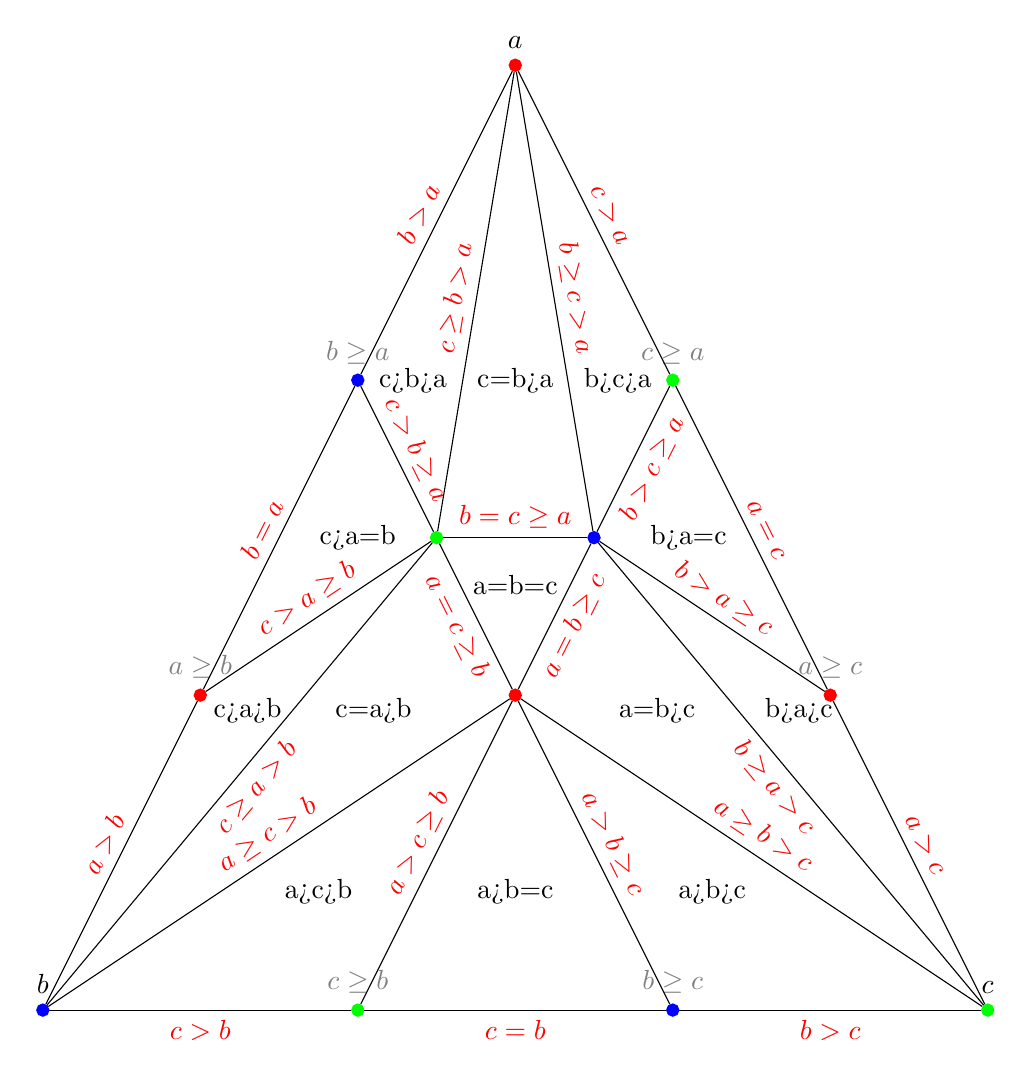
\begin{tikzpicture}
    \tikzstyle{red}=[circle,thick,draw=red,fill=red,inner sep=0pt,minimum width=4pt,minimum height=4pt]
    \tikzstyle{blue}=[circle,thick,draw=blue,fill=blue,inner sep=0pt,minimum width=4pt,minimum height=4pt]
    \tikzstyle{green}=[circle,thick,draw=green,fill=green,inner sep=0pt,minimum width=4pt,minimum height=4pt]
    \tikzstyle{point}=[circle,thick,draw=black,fill=black,inner sep=0pt,minimum width=4pt,minimum height=4pt]
    \node (a)[red,label={$a$}]     at (6,12) {};
    \node (b)[blue,label={$b$}]    at (0,0) {};
    \node (c)[green,label={$c$}]   at (12,0) {};
    \node (ab)[red,label={{\color{gray}$a \ge b $}}]    at (2,4) {};
    \node (ba)[blue,label={{\color{gray}$b \ge a $}}]   at (4,8) {};
    \node (ca)[green,label={{\color{gray}$c \ge a $}}]  at (8,8) {};
    \node (ac)[red,label={{\color{gray}$a \ge c $}}]    at (10,4) {};
    \node (cb)[green,label={{\color{gray}$c \ge b $}}]  at (4,0) {};
    \node (bc)[blue,label={{\color{gray}$b \ge c $}}]   at (8,0) {};

    \node (cba)[green] at (5,6) {};
    \node (bca)[blue]  at (7,6) {};
    \node (abc)[red]   at (6,4) {};
    \draw (a)   -- (ba)   node[pos=0.5,sloped,above] {{\color{red}$b>a$}};
    \draw (ba)  -- (ab)   node[pos=0.5,sloped,above] {{\color{red}$b=a$}};
    \draw (ab)  -- (b)    node[pos=0.5,sloped,above] {{\color{red}$a>b$}};
    \draw (b)   -- (cb)   node[pos=0.5,sloped,below] {{\color{red}$c>b$}};
    \draw (cb)  -- (bc)   node[pos=0.5,sloped,below] {{\color{red}$c=b$}};
    \draw (bc)  -- (c)    node[pos=0.5,sloped,below] {{\color{red}$b>c$}};
    \draw (c)   -- (ac)   node[pos=0.5,sloped,above] {{\color{red}$a>c$}};
    \draw (ac)  -- (ca)   node[pos=0.5,sloped,above] {{\color{red}$a=c$}};
    \draw (ca)  -- (a)    node[pos=0.5,sloped,above] {{\color{red}$c>a$}};
    \draw (ba)  -- (cba)  node[pos=0.5,sloped,above] {{\color{red}$c > b \ge a$}};
    \draw (ab)  -- (cba)  node[pos=0.5,sloped,above] {{\color{red}$c > a \ge b$}};
    \draw (cb)  -- (abc)  node[pos=0.5,sloped,above] {{\color{red}$a > c \ge b$}};
    \draw (bc)  -- (abc)  node[pos=0.5,sloped,above] {{\color{red}$a > b \ge c$}};
    \draw (ac)  -- (bca)  node[pos=0.5,sloped,above] {{\color{red}$b > a \ge c$}};
    \draw (ca)  -- (bca)  node[pos=0.5,sloped,below] {{\color{red}$b > c \ge a$}};
    \draw (a)   -- (cba)  node[pos=0.5,sloped,above] {{\color{red}$c \ge b > a$}};
    \draw (a)   -- (bca)  node[pos=0.5,sloped,above] {{\color{red}$b \ge c > a$}};
    \draw (b)   -- (cba)  node[pos=0.5,sloped,below] {{\color{red}$c \ge a > b$}};
    \draw (b)   -- (abc)  node[pos=0.5,sloped,above] {{\color{red}$a \ge c > b$}};
    \draw (c)   -- (abc)  node[pos=0.5,sloped,above] {{\color{red}$a \ge b > c$}};
    \draw (c)   -- (bca)  node[pos=0.5,sloped,below] {{\color{red}$b \ge a > c$}};
    \draw (cba) -- (bca)  node[pos=0.5,sloped,above] {{\color{red}$b = c \ge a$}};
    \draw (bca) -- (abc)  node[pos=0.5,sloped,below] {{\color{red}$a = b \ge c$}};
    \draw (abc) -- (cba)  node[pos=0.5,sloped,below] {{\color{red}$a = c \ge b$}};
    \node at (3.5,1.5) {a>c>b};
    \node at (6,1.5) {a>b=c};
    \node at (8.5,1.5) {a>b>c};
    \node at (2.6,3.8) {c>a>b};
    \node at (4.2,3.8) {c=a>b};
    \node at (6.0,5.4) {a=b=c};
    \node at (7.8,3.8) {a=b>c};
    \node at (9.6,3.8) {b>a>c};
    \node at (4.0,6.0) {c>a=b};
    \node at (8.2,6.0) {b>a=c};
    \node at (4.7,8.0) {c>b>a};
    \node at (6.0,8.0) {c=b>a};
    \node at (7.3,8.0) {b>c>a};
\end{tikzpicture}


\begin{tikzpicture}
\node (c)[circle,draw] at (0,0) {a=b=c};
\foreach \angle/\label in {0/{$b>a>c$},30/{$b>a=c$},60/{$b>c>a$},90/{$c=b>a$},120/{$c>b>a$},150/{$c>a=b$},180/{$c>a>b$},210/{$c=a>b$},240/{$a>c>b$},270/{$c>a>b$},300/{$a>b=c$},330/{$a>b>c$}}
\node[circle,draw] (\angle) at (\angle:5) {\label};
\foreach \node/\to in {210/240,210/270,210/300,210/330,240/300,240/330,270/330,60/90,90/120,120/60,0/30,150/180,240/270,270/300,300/330}
\draw (\node)  -- (\to)node;%[pos=0.5,sloped,above];// {{\color{red}$a$}};
\foreach \node in {210,240,...,330}
\draw (c)  -- (\node)node;%[pos=0.5,sloped,above] {{\color{red}$a$}};

\end{tikzpicture}


\subsections{Remarks}

In the construction of the simplicial complex:
\begin{itemize} 
\item Every node, it is a possible final state of a single process.
\item Every edge connects two nodes, for which there is a possible execution of events, they could simultaneously be the possible final state.
\item Every simplicial complex of dimmention n, connects n+1 nodes of n+1 different processes for which there is a possible execution where they could simultaneously be the possible final state.
\end{itemize}


\subsection{Kripke structures}

\subsubsection{Definition}\\

TODO.
\newpage

\subsubsection{Mapping}

We will use all possible executions (total orders) as worlds.\\

The accessibility relation will be always symetrical, (B)

\section{Specific objectives}

%----------------------------------------------------------------------------------------

\backmatter

%----------------------------------------------------------------------------------------
%	BIBLIOGRAPHY
%----------------------------------------------------------------------------------------

\bibliography{bibliography} % Use the bibliography.bib file for the bibliography
\bibliographystyle{plainnat} % Use the plainnat style of referencing

%----------------------------------------------------------------------------------------

%\printindex % Print the index at the very end of the document

\end{document}
